\section{Introduction}

% Applications like personalized medicine, meteorological forecasting, and natural language processing \pl{NLP is so broad...anything could go here; either motivate based on fields that already use calibration (good to stand on shoulders of giants) or say something substantive about why calibration is needed (danger of being too preachy (danger of being too preachy))} require that classifiers provide calibrated confidence measures in addition to their predictions~\cite{jiang2012calibrating, brocker2009decomposition, nguyen2015posterior}.
% In other words, the probability that a system outputs for an event should reflect the true frequency of that event: if an automated diagnosis system says 1,000 patient have cancer with probability 0.1, approximately 100 of them should indeed have cancer.
The probability that a system outputs for an event should reflect the true frequency of that event: if an automated diagnosis system says 1,000 patients have cancer with probability 0.1, approximately 100 of them should indeed have cancer.
In this case we say the model is uncertainty calibrated. The importance of this notion of calibration has been emphasized in personalized medicine~\cite{jiang2012calibrating}, meteorological forecasting~\cite{murphy1973vector, murphy1977reliability, degroot1983forecasters,gneiting2005weather, brocker2009decomposition} and natural language processing applications~\cite{nguyen2015posterior, card2018calibration}.
As most modern machine learning models, such as neural networks, do not output calibrated probabilities out of the box~\cite{guo2017calibration, zadrozny2001calibrated, kuleshov2018accurate}, recalibration methods take the output of an uncalibrated model, and transform it into a calibrated probability.
\emph{Scaling} approaches for recalibration---Platt scaling~\cite{platt1999probabilistic}, isotonic regression~\cite{zadrozny2002transforming}, and temperature scaling~\cite{guo2017calibration}---are widely used and require very few samples, but do they actually produce calibrated probabilities?
% , and speech recognition~\cite{dong2011calibration}
% These methods use additional recalibration data to fit a simple function on top of the original model outputs.

% Important, check that it's not too similar to "On calibration of modern neural networks" paper.
% In many applications, classification models must not only be accurate, but should indicate when they may be incorrect. For example, in automated healthcare applications, control should be passed on to human doctors when the confidence of a disease diagnosis prediction is low. Specifically, classifiers should provide a \emph{calibrated} confidence measure in addition to its prediction. In other words, the probability that a system outputs for an event should reflect the true frequency of that event: of the times that a system says a patient has cancer with probability 0.3, 30\% of the time, the patient should indeed have cancer.
% Typically, complex models like neural networks do not output calibrated probabilities.
% Instead, recalibration methods take the output of an uncalibrated model, and transform it into a calibrated probability.
% Popular recalibration approaches include Platt scaling and temperature scaling.

% Recent advances in machine learning have dramatically increased predictive accuracy. Machine learning methods are now entrusted with making decisions in applications ranging from weather forecasting to medical diagnosis \pl{seems a bit naive...}. In many of these settings, classification models must not only be accurate, but should indicate when they may be incorrect. For example, in automated healthcare applications, control should be passed on to human doctors when the confidence of a disease diagnosis prediction is low. Specifically, classifiers should provide a \emph{calibrated} confidence measure in addition to its prediction. In other words, the probability that a system outputs for an event should reflect the true frequency of that event: of the times that a system says that it will rain with probability 0.3,  30\% of the time, it should rain.
% \pl{need citations; is rain prediction really driven by "modern ML"?}\tm{It also seems unncessary to introduce the rain example --- it seems to be a good introduction to people who didn't know it before, but not something to write in the first para of a paper?}

%  \pl{I'd try to combine with first paragraph so that it's all background}
% \pl{introduce calibration error as a central concern first;
% methods try to calibrate, but do they actually achieve it?
% }

\emph{We discover that these methods are less calibrated than reported.} Past work approximates a model's calibration error using a finite set of bins. We show that by using more bins, we can uncover a higher calibration error for models on CIFAR-10 and ImageNet.
We show that a fundamental limitation with approaches that output a continuous range of probabilities is that their true calibration error may never be measurable with a finite number of bins (Example~\ref{ex:continuous-not-calibrated}).

An alternative approach, histogram binning~\cite{zadrozny2001calibrated}, outputs probabilities from a finite set.
Histogram binning can produce a model that is calibrated, and unlike scaling methods we can measure its calibration error, but it can be \pl{is (try to use simple verbs whenever posible, though not always possible)} sample inefficient.
In particular, the number of samples required to calibrate scales linearly with the number of distinct probabilities the model can output, $B$~\cite{naeini2014binary}, which can be large particularly in the multi-class \pl{multiclass} setting where $B$ typically scales with the number of classes.
Recalibration sample efficiency is crucial -- \pl{---} we often want to recalibrate our models in the presence of domain shift~\cite{hendrycks2019anomaly} or recalibrate a model trained on simulated data, and may have access to only a small labeled dataset from the target domain.

To get the sample efficiency of Platt scaling and the verification guarantees of histogram binning, \emph{we propose the variance-reduced calibrator} (Figure~\ref{fig:var_red_binning}).
Like scaling methods, we fit a simple function $g \in \mathcal{G}$ to the recalibration dataset.
We then bin the input space so that an equal number of inputs land in each bin.
In each bin, we output the average of the $g$ values in that bin---these are the gray circles in Figure~\ref{fig:var_red_binning}.
In contrast, histogram binning outputs the average of the label values in each bin (Figure~\ref{fig:hist_binning}).
The motivation behind our method is that the $g$ values in each bin are in a narrower range than the label values, so when we take the average we incur less of an estimation error.
If $\mathcal{G}$ is well chosen, our method requires $O(\frac{1}{\epsilon^2} + B)$ samples to achieve calibration error $\epsilon$ instead of $O(\frac{B}{\epsilon^2})$ samples for histogram binning, where $B$ is the number of model outputs (Theorem~\ref{thm:final-calib}). Note that in prior work\pl{,} binning the outputs of a function was used for evaluation and without any guarantees, whereas in our case it is used for the method itself and we show improved sample complexity.

% As with other recalibration methods, we begin with a recalibration dataset $\{(z_1, y_1), ..., (z_n, y_n)\}$, where $z_i$ represents the uncalibrated model output and $y_i$ the ground truth label.
% In the binary classification setting, $z_i \in [0, 1]$ and $y_i \in \{0, 1\}$.
% We fit a simple function $g \in \mathcal{G}$ to the recalibration dataset.
% We then bin the input space so that an equal number of $g(z_i)$ land in each bin.
% In each bin, we output the average of the $g(z_i)$ values in that bin -- these are the gray circles in Figure~\ref{fig:var_red_binning}.
% Binning ensures that the output probabilities are from a finite set, so we can check if it is calibrated.
% In contrast, histogram binning takes the average of the $y_i$ values in each bin (Figure~\ref{fig:hist_binning}).
% The motivation behind our method is that the $g(z_i)$ values in each bin are in a narrower range than the $y_i$ values -- when we take the average we incur less of an estimation error.
% If $\mathcal{G}$ is well chosen, our method requires $O(\frac{1}{\epsilon^2})$ samples to achieve calibration error $\epsilon$ instead of $O(\frac{B}{\epsilon^2})$ samples for histogram binning, where $B$ is the number of model outputs (Theorem~\ref{thm:final-calib}).
% \pl{this is good overall, but I wonder if it's too much setup / notation from the intro, and it's strange that it's introduced for our method and not the general problem setting}

\begin{figure}
     \centering
     \begin{subfigure}[b]{0.32\textwidth}
         \centering
         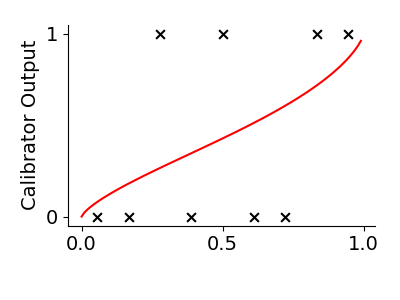
\includegraphics[width=\textwidth]{platt_scaling}
         \caption{Platt scaling.}
         \label{fig:platt_scaling}
     \end{subfigure}
     \hfill
     \begin{subfigure}[b]{0.32\textwidth}
         \centering
         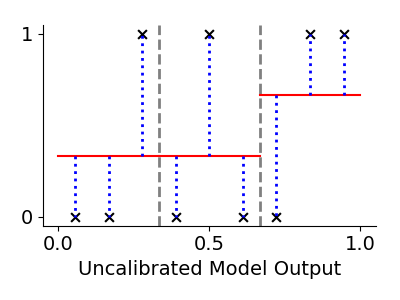
\includegraphics[width=\textwidth]{histogram_binning_with_deltas}
         \caption{Histogram binning.}
         \label{fig:hist_binning}
     \end{subfigure}
     \hfill
     \begin{subfigure}[b]{0.32\textwidth}
         \centering
         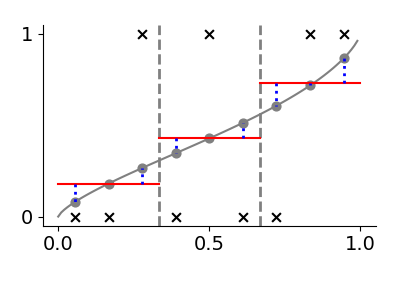
\includegraphics[width=\textwidth]{variance_reduced_binning_with_deltas}
         \caption{Variance-reduced calibrator.}
         \label{fig:var_red_binning}
     \end{subfigure}
        \caption{
        Visualization of the 3 recalibration approaches.
        The black crosses are the ground truth labels, and the red lines are the output of the recalibration methods.
        Platt Scaling (Figure~\ref{fig:platt_scaling}) fits a function to the recalibration data, but its calibration error is not measurable.
        Histogram binning (Figure~\ref{fig:hist_binning}) outputs the average label in each bin.
        Our variance-reduced calibrator (Figure~\ref{fig:var_red_binning}) fits a function $g \in \mathcal{G}$ to the recalibration data and then \emph{takes the average of the function values (the gray circles)} in each bin.
        The function values have lower variance than the labels, as visualized by the blue dotted lines, which is why our approach has lower variance. 
        }
        \label{fig:variance_reduced_illustration}
\end{figure}

\pl{don't ask rhetorical question since this already has an answer, we are just improving on it; say: 'Next, we turn to the question of estimating the calibration error'}
How do we check if the model produced by a recalibration method is actually calibrated? This is an important problem because all methods may achieve calibration error lower or higher than their theoretical rates predict---\cite{hendrycks2019anomaly} measures calibration error when the test distribution is different from train, where this is especially true. \pl{do we really need to justify this? seems uncontroversial to me} Prior work in machine learning~\cite{nguyen2015posterior, guo2017calibration, hendrycks2019anomaly, kuleshov2015calibrated, hendrycks2019pretraining} directly estimates each term in the calibration error from samples (Definition~\ref{dfn:plugin-estimator}).
The sample complexity of this plugin estimator scales linearly with $B$.
\emph{We show that an alternative estimator introduced in the meteorological literature~\cite{brocker2012empirical, ferro2012bias} has sample complexity that scales with $\sqrt{B}$ (Theorem~\ref{thm:final-ours})}.
\pl{make it more clear that we proved a result here;
I'd say---this other estimator removes bias; we show that it actually obtains $\sqrt{B}$
}
We prove that it achieves this by leveraging error cancellations across bins.

We run multi-class \pl{multiclass} calibration experiments on CIFAR-10~\cite{krizhevsky2009learningmultiple} and ImageNet~\cite{deng2009imagenet}.
The objective is to minimize the mean-squared error, also known as the Brier score~\cite{brier1950verification}, subject to a calibration error budget~\cite{gneiting2005weather}.
We show that the variance-reduced calibrator achieves a better calibration error than histogram binning, while allowing us to measure the true calibration error.
For example, we get a \emph{35\% lower calibration error on CIFAR-10} than histogram binning if $B = 100$.

% In summary, our contributions are:
% \begin{enumerate}
% \item We show that scaling methods for recalibration are less calibrated than reported.
% \item We propose variance-reduced calibration which has the sample complexity of scaling methods, but we can actually verify its calibration.
% \item We show that the method typically used to estimate calibration error is suboptimal, and an alternative estimator requires fewer samples to measure the calibration error.
% \end{enumerate}

\tm{Sometimes I do a summary of contribution paragraph for the reviewers to easily see the contribution. doesn't add anything to the quality of the paper, but sometimes useful for paper acceptance .. (As a rushed reviewer sometimes I wanted the authors to have a simple para with a bit more technical term than abstract....)}

\pl{it's a nice to have if we have space; the use of italics throughout the intro is actually pretty effective}
